\section{Development Environment}
\subsection{Platform, Languages, and Cost}
\subsubsection{PC and server platforms}
Linux is the first client target because it offers direct camera/microphone access and a common GStreamer pipeline for controlled playback and capture. Python is selected for application logic and server inference; PySide6 provides the desktop interface, and PyGObject connects the client to GStreamer. Asynchronous acquisition and inference prevent a slow network or model from blocking sensor controls. The reproducible client target is Ubuntu 24.04 LTS, Python 3.12, PySide6 6.8.3, GStreamer 1.24, and FFmpeg 6.1. These are selected integration baselines, not a claim that the application already runs on them.

The inspected workstation runs Ubuntu 26.04.1 LTS on an AMD Ryzen AI 7 350 with 8 cores/16 threads and approximately 14.2~GiB of OS-visible RAM. The client will be tested in its specified environment before distribution; host-installed packages are not the dependency lock. Webcam and microphone models will be recorded during the capture trial. The plan assumes existing equipment, not a new PC or GPU purchase.

The AWS target is one Linux \code{g4dn.xlarge} in Asia Pacific (Seoul): 4 vCPUs, 16~GiB RAM, and one NVIDIA T4 with 16~GiB GPU memory~\cite{ec2spec}. An 80~GB encrypted gp3 EBS volume holds the database, model files, and bounded temporary analysis data. Durable records do not depend on instance-store survival. Docker Compose runs the API, queue, database, and inference services on this host. One resident audio model uses the GPU; facial analysis initially uses CPU within the inference service. This preserves server-side audio and video analysis without duplicating GPU model allocations. Load measurements will determine whether concurrency or instance size must change.

\subsubsection{Software baseline}
The server target is Ubuntu 24.04 LTS with separate Python 3.11 environments for the API and inference worker. Proposed pins are FastAPI 0.162.0, PyTorch 2.9.1 with CUDA 12.6, MediaPipe 0.10.21, and NumPy 1.26.4 in the worker. Redis 7.2 provides a bounded work stream; PostgreSQL 16 stores sessions, events, result cursors, and deletion state. Docker Engine 28 and Compose 2 are the server packaging baseline. Exact patch versions, image digests, compatible NVIDIA driver/container-toolkit versions, model checksums, and the PANNs source revision will be locked after clean installation and an end-to-end inference trial. A dependency lock alone does not prove model or media compatibility.

\subsubsection{Estimated expenditure}
The estimate uses Linux shared-tenancy On-Demand pricing in Seoul, checked November 4, 2026: \$0.647 per GPU-instance hour, \$0.0912 per GB-month of gp3 storage, and \$0.005 per public IPv4 address-hour~\cite{ec2price,ipv4}. For 80~GB-month of EBS and one retained IPv4 address for 720 hours,
\begin{equation}
 C(h)=0.647h+80(0.0912)+720(0.005).
\end{equation}
Thus 40, 80, and 120 active GPU hours cost \$36.78, \$62.66, and \$88.54, respectively, before credits and tax. EBS and an allocated public address can incur charges while the instance is stopped. This excludes paid data transfer beyond applicable allowances, extra storage, paid monitoring, and subsequently purchased devices or licenses.

Existing equipment is budgeted at \$0 incremental hardware cost. No paid development-tool subscription or model-training service is planned. Distribution must retain applicable software and model-license notices; PANNs code and pretrained weights have distinct licenses~\cite{panns,pannsweights}. No managed Kubernetes control-plane charge is included. New-account Free Tier credits are intended to offset eligible usage; actual account plan, remaining credit, GPU quota, and expiry are unverified. GPU capability remains in the design even if eligibility requires another funding arrangement~\cite{freetier}.

\begin{table*}[!t]
\caption{Selected Development Baseline (Integration Validation Pending)}
\label{tab:baseline}
\centering
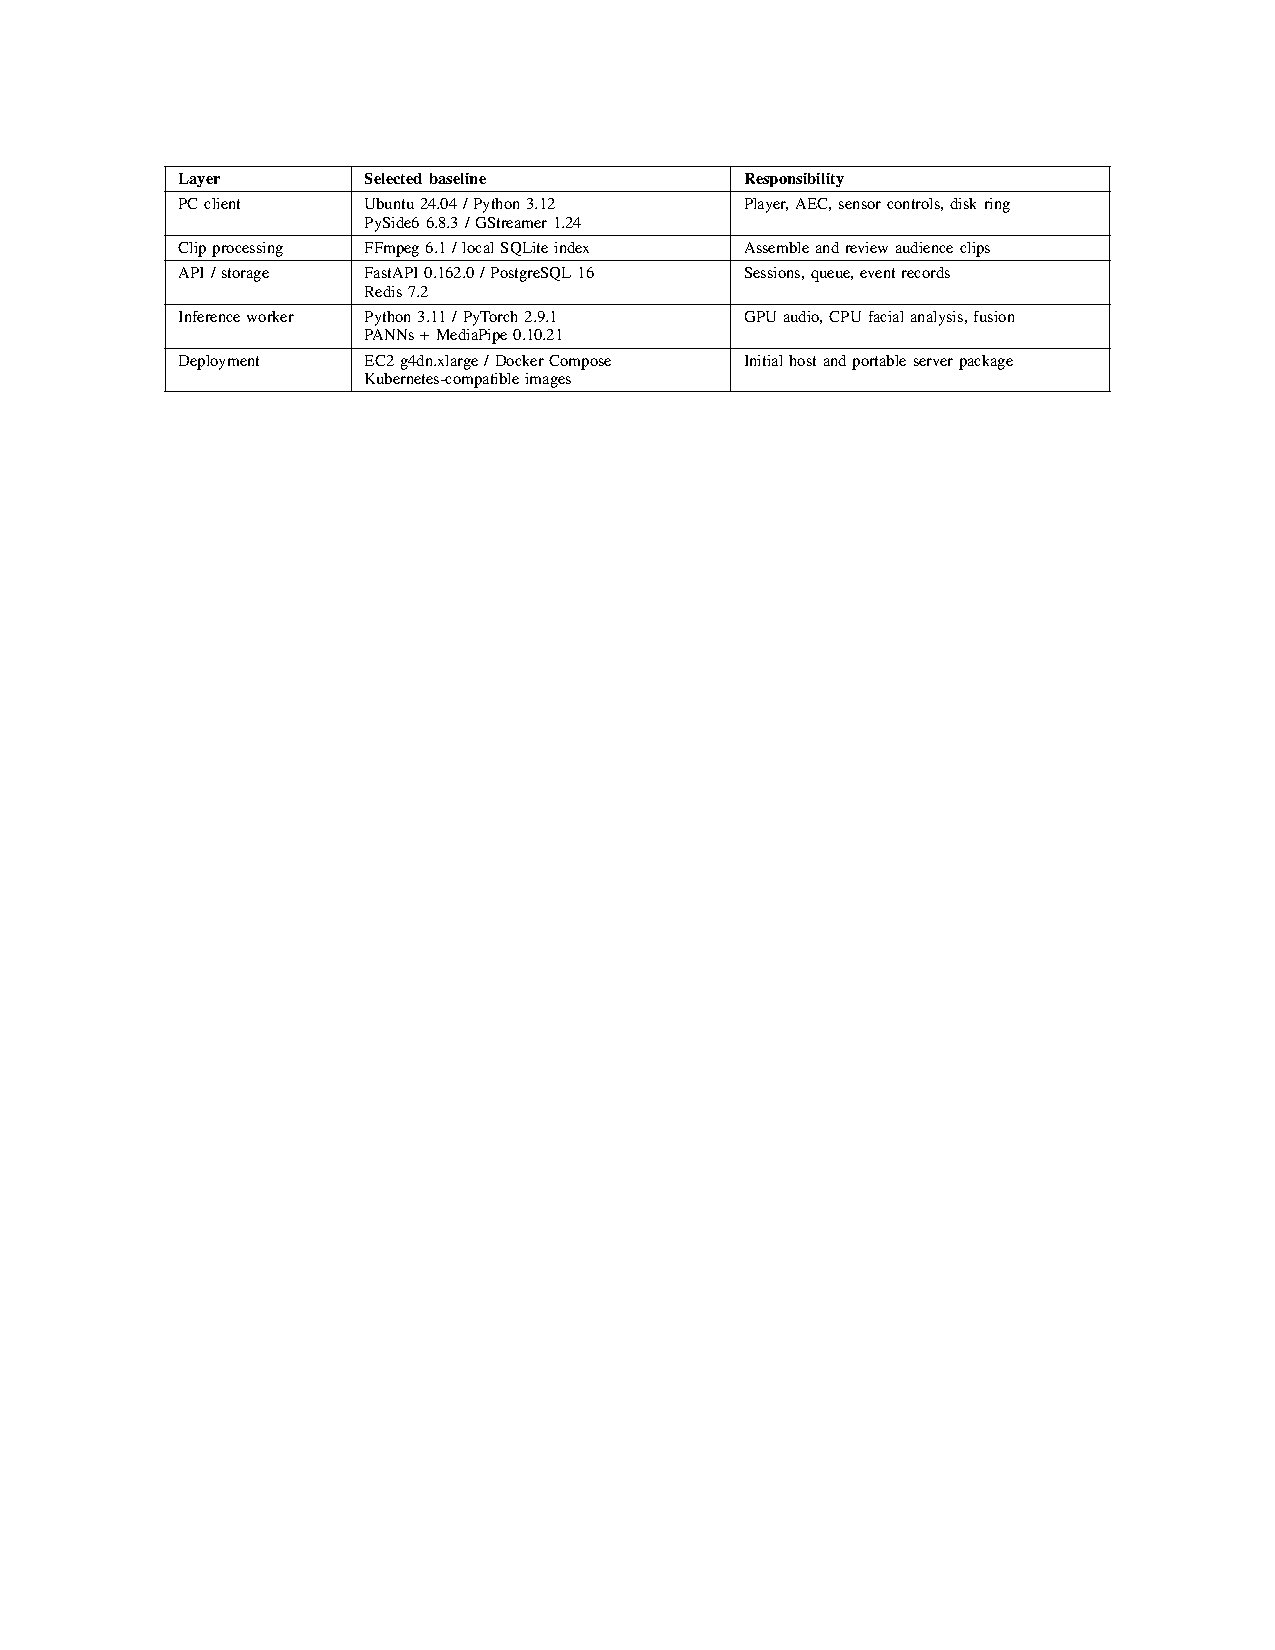
\includegraphics[width=\textwidth]{images/development-baseline.pdf}
\end{table*}

\subsection{Software and Processing Choices}
Table~\ref{tab:baseline} summarizes the selected layers and responsibilities.
GStreamer routes decoded player PCM through \code{webrtcechoprobe} before speaker output, while \code{webrtcdsp} processes microphone input in the same top-level pipeline. The probe is created before the DSP input becomes active; both branches use the same sample rate~\cite{gst-aec}. This is local signal preprocessing; reaction inference remains on the server. Camera video is split into independently decodable segments for the disk buffer. A reduced-resolution branch supplies analysis frames. FFmpeg assembles selected local segments into a reviewable clip, without uploading continuous original footage.

The initial audio candidate is PANNs \code{Cnn14\_DecisionLevelMax}, its pretrained AudioSet checkpoint, and 32~kHz mono input~\cite{panns,pannsweights}. Time-resolved output is mapped to capture timestamps. ``Screaming,'' ``Laughter,'' and ``Gasp'' map to the required classes. MediaPipe supplies per-face observations~\cite{mediapipe}; track identifiers are session-local and do not identify people. A single room microphone does not establish speaker-to-face identity. Classification confidence, observable intensity, and facial evidence remain distinct quantities.

The API accepts timestamped packets and places references to bounded temporary payloads into Redis Streams. Workers acknowledge jobs after event/result transactions commit. Stable keys make retries idempotent; at-least-once delivery is not exactly-once inference~\cite{redis}. The PC stores its clip index and result cursor in SQLite; PostgreSQL stores server event state. Saved clips remain local in this baseline. Server payloads expire after processing or a bounded retention interval; expiry produces an explicit dropped-input status.

\subsection{Responsibilities and Iterative Process}
The existing roles are retained. Soyeon Seol develops the PC interface and represents the User role; Pavel Kim develops backend/session/record services and represents the Customer role; Yujeong Heo develops AEC integration, audio recognition, and intensity evaluation; Chul Park manages development, media buffering/transport, and deployment integration. Facial-analysis integration is planned with AI/media work and needs a named issue owner before implementation. All members review requirement coverage and integration.

GitHub Issues and Projects will manage work beside source and pull requests~\cite{projects}. The proposed process uses one-week timeboxes, relative estimates, and capacity agreed at planning. This cadence is a project choice, not a lecture-mandated duration. Each issue identifies a Requirement number, acceptance case, owner, reviewer, estimate, and iteration. Board states are Backlog, Ready, In Progress, Review, and Done. Each developer begins with one active implementation task; blocked work is discussed before taking another.

At a brief daily check-in, members report completed work, today's work, blockers, omissions, and useful learning; problem solving follows separately. This follows the lectures' story/task planning, stand-up questions, and continuous integration guidance~\cite{lifecycle,management}. Weekly demonstrations with the User and Customer representatives drive reprioritization, followed by a short retrospective. Unfinished work returns to planning. Requirement changes require explicit review rather than silent removal to fit a sprint.

The first increment connects player reference, PC capture, server recognition, and a returned event. Later increments add clips/review, then failure handling and deployment checks. Good-to-have requirements are scheduled only after every must-have requirement passes its acceptance case. Integration and documentation target the recorded December 3, 2026 development milestone. Weekly scope follows demonstrated capacity. A task is Done when its acceptance case passes, a teammate reviews it, and the merged build works. CI will run unit/contract tests, supported media-fixture tests, container builds, and LaTeX compilation. Hardware/GPU checks run on the corresponding device, with evidence linked to the issue. Expected outcomes for AI-generated code are reviewed independently of that code.
